\documentclass{article}
\usepackage[utf8]{inputenc}
\usepackage{amsmath}
\usepackage{systeme}
\usepackage[most]{tcolorbox}
\usepackage[scale=.95,type1]{cabin}
\usepackage{lmodern}

\usepackage[legalpaper,margin=1in]{geometry}

\setlength{\parindent}{10pt}
\setlength{\parskip}{1em}
\renewcommand{\baselinestretch}{1.2}

\title{Matrices}
\date{}

\newcounter{example}[section]
\newenvironment{example}[1][]{\refstepcounter{example}\par\medskip
   \noindent \textbf{Example~\theexample. #1} \rmfamily}{\medskip}

\makeatletter
\renewcommand*\env@matrix[1][*\c@MaxMatrixCols c]{%
  \hskip -\arraycolsep
  \let\@ifnextchar\new@ifnextchar
  \array{#1}}
\makeatother

\newcommand\y{\cellcolor{blue!10}}
\newcommand\B{\textbf}

\usepackage{tabularray}
\SetTblrInner{colsep=5pt,rowsep=1pt}

\newcommand\x{\times}

\makeatletter
\newcommand{\dashover}[2][\mathop]{#1{\mathpalette\df@over{{\dashfill}{#2}}}}
\newcommand{\fillover}[2][\mathop]{#1{\mathpalette\df@over{{\solidfill}{#2}}}}
\newcommand{\df@over}[2]{\df@@over#1#2}
\newcommand\df@@over[3]{%
  \vbox{
    \offinterlineskip
    \ialign{##\cr
      #2{#1}\cr
      \noalign{\kern1pt}
      $\m@th#1#3$\cr
    }
  }%
}
\newcommand{\dashfill}[1]{%
  \kern-.5pt
  \xleaders\hbox{\kern.5pt\vrule height.4pt width \dash@width{#1}\kern.5pt}\hfill
  \kern-.5pt
}
\newcommand{\dash@width}[1]{%
  \ifx#1\displaystyle
    2pt
  \else
    \ifx#1\textstyle
      1.5pt
    \else
      \ifx#1\scriptstyle
        1.25pt
      \else
        \ifx#1\scriptscriptstyle
          1pt
        \fi
      \fi
    \fi
  \fi
}
\newcommand{\solidfill}[1]{\leaders\hrule\hfill}
\makeatother

\begin{document}
    \section{Operations with Matrices}

    Denote matrix : $ \begin{cases}{}
        A, B, C, \dots \text{ or  } [a_{ij}], [b_{ij}], [c_{ij}] \\
        \text{A rectangular array of numbers} \begin{bmatrix}
            a_{11} & a_{12} & \dots & a_{1n} \\
            a_{21} & a_{22} & \dots & a_{2n} \\
            \vdots & \vdots & \ddots & \vdots \\
            a_{m1} & a_{m2} & \dots & a_{mn}
        \end{bmatrix}
    \end{cases}$

    \begin{tcolorbox}
        \bf{Equality of Matrices.} 
        \[ A = [a_{ij}] = [b_{ij}] = B \] for all $1 \leq i \leq m$  and $1 \le j \le n$
    \end{tcolorbox}

    \begin{itemize}
        \item Column matrix - Column vector 
            $\begin{bmatrix}
                1 \\
                3
            \end{bmatrix}$
        \item Row matrix - Row vector
            $ \begin{bmatrix}
                1 & 3
            \end{bmatrix}$
    \end{itemize}

    \subsection*{\textcolor{blue}{Matrix Addition}}
        \begin{tcolorbox}
            $A + B = [a_{ij} + b_{ij}]$
        \end{tcolorbox}

    \subsection*{\textcolor{blue}{Scalar Multiplication}}
        \begin{tcolorbox}
            \[ cA = [ca_{ij}] \]
        \end{tcolorbox}

    \subsection*{\textcolor{blue}{Matrix Multiplication}}

    \begin{tcolorbox}
        $A = [a_{ij}]$ is an $m \x n$ matrix and $B = [b_{ij}]$ is an $n \x p$ matrix, then the \textbf{product} AB
        is an $m \x p$ matrix : $AB = [c_{ij}]$ \\
        use the $i^{\text{th}}$ row of $A$ and the $j^{\text{th}}$ column of $B$  \[ c_{ij} = \sum_{k=1}^{n} a_{ik}b_{kj} \]
    \end{tcolorbox}

    \begin{itemize}
        \item not \B{commutative} : $AB$ is not always equal to $BA$
    \end{itemize}
    
    \subsubsection*{Systems of Linear Equations}

    $A$ : the coefficient matrix of the system\\
    \B{x} and \B{b} are column matrices.

    Rewrite the system as 
    $  \underset{A}{\begin{bmatrix}
        a_{11} & a_{12} & a_{13} \\
        a_{21} & a_{23} & a_{23} \\
        a_{31 } & a_{32} & a_{33}
    \end{bmatrix}
}
    \underset{x}{\begin{bmatrix}
        x_1 \\ x_2 \\ x_3
    \end{bmatrix}
}    = \underset{b}{\begin{bmatrix}
        b_1 \\ b_2 \\ b_3
    \end{bmatrix}}$

    \subsubsection*{Partitioned Matrix}
    \[b = x_1 \begin{bmatrix}
        a_{11} \\ a_{21} \\ \vdots \\ a_{m1}  \end{bmatrix} + \dots + x_n\begin{bmatrix}
            a_{1n} \\ a_{2n} \\ \vdots \\ a_{mn}
           \end{bmatrix} = \sum_{j=1}^{n} x_{j}a_{j} \]

    That is, a \textbf{linear combination} of the column matrices \B{$a_1, a_2, \dots, a_n$} 
    with \B{coefficients} $x_1, x_2, \dots, x_n$

    \subsection*{Properties of Matrix Operations}
    \begin{enumerate}
        \item $-A$ : \B{additive inverse} of $A$
        \item $A + B = B + A$ (Commutative property of addition)
        \item $A + (B + C) = (A + B) + C$ (Associative property of addition)
        \item $(cd)A = c(dA)$ (Associative property of multiplication)
        \item $IA = A$ (Multiplicative identity)
        \item $c(A + B) = cA + cB$ (Distributive property)
        \item $(c+ d)A = cA + dA$ (Distributive property)
    \end{enumerate}

    \subsection*{Properties of Matrix Multiplication}
    \begin{enumerate}
        \item not having general cancellation:  $AC = BC$ doesn't mean $A = B$
        \item $AB$ is not always equal to $BA$
        \item $(AB)C = A(BC)$ 
        \item $A(B + C) = AB + AC$
        \item $(A + B)C = AB + AC$
        \item $c(AB) = A(cB)$
    \end{enumerate}

    \subsubsection*{Identity Matrix of order $n$}
    $ I_n = \begin{bmatrix}
        1 & 0 & \dots & 0 \\
        0 & 1 & \dots & 0 \\
        \vdots & \vdots & \ddots & \vdots \\
        0 & 0 & \dots & 1
    \end{bmatrix}$
    \begin{tcolorbox}
        $A$ is a $m \x n$ matrix :
        $AI_n = A$ \\
        $I_mA = A$
    \end{tcolorbox}
    
    \subsubsection*(The Transpose of a Matrix)

    The \B{transpose} of a matrix is formed by writing its columns as rows. 

    \[ A = \begin{bmatrix}
        a_{11} & a_{12} & \dots  & a_{1n} \\
        \vdots &  &  & \\
        a_{m1} & a_{m2} & \dots & a_{mn}
    \end{bmatrix} \text{ then  }  \quad A^{T} = \begin{bmatrix}
        a_{11} & a_{21} & \dots & a_{m1} \\
        \vdots  & &  & \\
        a_{1n} & a_{2n} & \dots  & a_{mn}
    \end{bmatrix} \]

    \begin{tcolorbox}
        \begin{enumerate}
            \item $(A^T)^T =   A$
            \item $(A + B)^T = A^T + B^T$
            \item $(ABC)^T = C^T.B^T.A^T$ 
            \item $(AA^T) = (AA^T)^T = (A^T)^T.A^T$. So $AA^T$ is symetric.
        \end{enumerate}
    \end{tcolorbox}

    \subsection*{The Inverse of A Matrix}
    \begin{tcolorbox}
        An $n \x n$ matrix is \B{invertible} (or \B{nonsingular}) if there exists an $n \x n$ matrix $A^{-1}$
        such that \[ AA^{-1} = A^{-1}A = I_n\]
    \begin{itemize}
        \item $A^{-1}$ : the (multiplicative) \B{inverse} of $A$
        \item Else, $A$ is \B{noninvertible} (or \B{singular})
        \item $A^{-1}$ is \B{unique}
    \end{itemize}
    \end{tcolorbox}
    If $AB = I_n$, it can be shown that $BA = I_n$ as well.

    \subsection*{Finding the Inverse of a Matrix}

    \B{Notice: } The column vectors $a_1, a_2, \dots, a_n$ have the same coefficient matrix which is
    $A$. 
    \[ \begin{bmatrix}[cc|cc]
        1 & 4 & 1 & 0\\
        -1 & -3 & 0 & 1
    \end{bmatrix}
    \to \begin{bmatrix}[cc|cc]
        1 & 0 & -3 & -4 \\
        0 & 1 & 1 & 1
    \end{bmatrix}\]

    \[ [A \vdots I] \to [I \vdots A^{-1}]\]
    If A can't be row reduced to $I_n$, then A is \B{noninvertible} (or \B{singular})
    
    \begin{tcolorbox}
    For $2 \x 2$ matrix
    \[ A = \begin{bmatrix}
        a & b \\
        c & d
    \end{bmatrix} \text{ then  } \quad A^{-1} = \frac{1}{ad - bc} \begin{bmatrix}
        d & -b \\
        -c & a
    \end{bmatrix} \]
    The determinator $ad - bc$ : the \B{determinant} of $A$.
    \end{tcolorbox}
    

    \begin{tcolorbox}[width=\textwidth,colback={blue9}]    
       \begin{enumerate}
           \item  $(A^{-1})^{-1} = A$
           \item $(A^k)^{-1} = A^{-1}.A^{-1}\dots A^{-1} = (A^{-1})^k$
           \item $(cA)^{-1} = \frac{1}{c} A^{-1}, c \neq 0$
           \item $(A^T)^{-1} = (A^{-1})^{T}$
           \item If $A$ and $B$ are \B{invertible}, then $AB$ is \B{invertible} : $(AB)^{-1} = B^{-1}A^{-1}$ \\
               Thus, reverse the order of multiplication to find the inverse
               \[ (A_1A_2\dots A_n)^{-1} = A_n^{-1}A_{n-1}^{-1}\dots A_1^{-1}\]
           \item If \B{$C$ is invertible matrix} 
               \[ AC = BC \Leftrightarrow A = B \]
               \[ CA = CB \Leftrightarrow A = B \]  
       \end{enumerate} 
    \end{tcolorbox}   

    \subsection*{Systems of Equations}
    For \textit{square} systems (those having the same number of Eq. as variables), you can use the 
    theorem below to determine whether the system has a \B{unique solution}.
    
    \begin{tcolorbox}[width=\textwidth,colback={blue9}]    
        If $A$ is invertible,then the linear equation $Ax = b$ has an unique solution
        $x = A^{-1}b$
    \end{tcolorbox}   

    \section{Elementary Matrices}


    \begin{tcolorbox}[width=\textwidth,colback={blue9}]    
        \begin{enumerate}
            \item \B{Elementary matrix} $E$ : can be obtained from $I_n$ by \B{1 elementary row operation}.
        If that same operation is performed on $A_{m \x n}$ , the resulting matrix is given
        by the product $EA$.
        \item Matrix $B$ is \B{row-equivalent} to $A$ if there exists a finite number of elementary
        matrices $E_1, E_2, \dots, E_k$ such that 
        \[ B = E_1E_2\dots E_k A\]
        \item $E^{-1}$ exist and is an \B{elementary matrix}. The \B{inverse} $E^{-1}$ is simply found by
            reverse the operation to get $E$.
        \end{enumerate}
        \end{tcolorbox}   

    \begin{center}
    \begin{tcolorbox}[hbox,    %%<<---- here
           lifted shadow={1mm}{-2mm}{3mm}{0.1mm}%
           {black!50!white}]
           $A$ is \B{invertible} $\Leftrightarrow A = E_1E_2\dots E_k$
    \end{tcolorbox}
    \end{center}
    Consider the \B{homogeneous S. Eq} represented as $Ax = O$. Since $A$ is invertible, it 
    only has the \B{trivial solution}. But this implies that the \B{augmented matrix} 
    $[A \vdots O]$ can be rewritten in the form $[I \vdots O]$  using $E_1, E_2, \dots, E_k$.
        
    We now have $E_k \dots E_2E_1A = I$. It follows that $A = E_1^{-1}E_2^{-1}\dots E_k^{-1}$.

    \subsection*{\textcolor{blue3}{Equivalent Conditions}}

    \begin{center}
    \begin{tcolorbox}
           If $A$ is an $n \x n$ matrix, the following statements are equivalent.
           \begin{enumerate}
               \item $A$ is \B{invertible}
               \item $Ax = b$ has a unique solution for every $n \x 1$ column matrix $b$.
               \item $Ax = O$ has only the trivial solution.
               \item $A$ is \B{row-equivalent} to $I_n$
               \item $A$ can be written as the product of elementary matrices.
           \end{enumerate}
    \end{tcolorbox}
    
    \end{center}

    \section{The LU-Factorization}
    
    At the heart of the most efficient and modern algorithms for solving linear systems,
    $Ax = b$ is the so-called $LU$-factorization, in which the square matrix $A$ is expressed as
    a product $A = LU$.

    $ \begin{array}{cc}
        \begin{bmatrix}
            a_{11} & 0 & 0 \\
            a_{21} & a_{22} & 0 \\
            a_{31} & a_{32} & a_{33}
        \end{bmatrix}
        & \begin{bmatrix}
            a_{11} & a_{12} & a_{13} \\
            0 & a_{22} & a_{23} \\
            0 & 0 & a_{33}
        \end{bmatrix} \\
        L:\text{ lower triangular matrix } & U:\text{ upper triangular matrix }
    \end{array}$

    By writing $Ax = LUx$ and letting $Ux = y$, you can solve $x$ for 2 stages:
    \begin{enumerate}
        \item Solve $Ly = b$ for $y$
        \item Solve $Ux = y$ for $x$
    \end{enumerate}

    
    \subsection*{Finding the LU-Factorizations of a Matrix}

    Find the $LU$-factorization of $A = \begin{bmatrix}
        1 & -3 & 0 \\
        0 & 1 & 3 \\
        2 & -10 & 2
    \end{bmatrix}$

    \begin{center}
        \begin{tabular}{c c c}
        \text{\textit{\textcolor{blue}{Matrix}}} & \text{\textit{\textcolor{blue}{Elementary Row Operation}}}
        & \text{\textit{\textcolor{blue}{Elementary Matrix}}}\\
        $\begin{bmatrix}
            1 & -3 & 0\\
            0 & 1 & 3 \\
            0 & -4 & 2
        \end{bmatrix}$ &
        $R_3 + (-2)R_1 \to R_3$ &
        $E_1 = \begin{bmatrix}
            1 & 0 & 0 \\
            0 & 1 & 0 \\
            -2  & 0 & 1
        \end{bmatrix}$ \\
        $\begin{bmatrix}
            1 & -3 & 0 \\
            0 & 1 & 3 \\
            0 & 0 & 14
        \end{bmatrix}$ &
        $R_3 + (4)R_2 \to R_3 $ &
        $E_2 = \begin{bmatrix}
            1 & 0 & 0 \\
            0 & 1 & 0 \\
            0 & 4 & 1
        \end{bmatrix} $
        \end{tabular}
    \end{center}

    The matrix $U$ on the left is upper triangular, and $E_2E_1A = U$, or $A = E_1^{-1}E_2^{-1}U$ . Because
    the product of lower triangular matrices 
    \[ E_1^{-1}E_2^{-1} = \begin{bmatrix}
            1 & 0 & 0 \\
            0 & 1 & 0 \\
            2  & 0 & 1
        \end{bmatrix}\begin{bmatrix}
            1 & 0 & 0 \\
            0 & 1 & 0 \\
            0 & -4 & 1
        \end{bmatrix} = \begin{bmatrix}
            1 & 0 & 0 \\
            0 & 1 & 0 \\
            2 & -4 & 1
        \end{bmatrix} \]
    is again a lower triangular matrix $L$, the factorization $A = LU$ complete.
    
    Note that the multipliers are negatives of the corresponding entries in $L$. If
    $U$ is obtained from $A$ using row operation of adding a multiple of 1 row to 
    another row below, then $L$ is a lower triangular matrix with 1's along the 
    diagonal. Furthermore, the negative of each multiplier is the same position
    as that of the corresponding zero in $U$.

    \begin{enumerate}
        \item Write $y = Ux $ and solve $Ly = b$ for $y$.
        \item Solve $Ux = y$ for $x$.
    \end{enumerate}
    Those steps are just \B{forward-substitution} and \B{back-substitution}, since it's
    all triangular matrices.

    \section{Applications of Matrix Operations}

    \subsection{Stochastic Matrices}

    Give a finite set of \textit{states} ${S_1, S_2, \dots, S_n}$.\\
    {\footnotesize \textit{For instance, residents of a city may live downtown or in the suburbs. Voters may vote Democrat, Republican, or for a third party. Soft drink consumers may buy Coca-Cola, Pepsi Cola, or another brand.}
    $\bullet 0 \leq p_{ij} \leq 1$ : the probability that a member will change from the $j$th state to the $i$th state.
    
    \begin{center}
    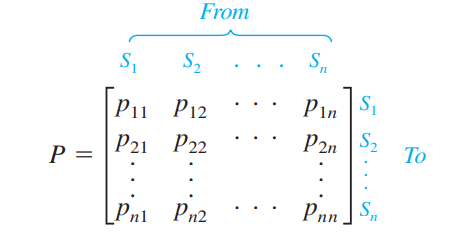
\includegraphics[width = 6cm]{ptransition.png}
    \end{center}

    $P$: \B{matrix of transition probabilities}, since it gives the probabilities of each possible type
    of transition.

    At each transition, each member in a given state $ \begin{cases}{}
        \text{stay in that state} \\ \text{change to another state}
    \end{cases}$

    This means the sum of the entries in any column of $P$ is $1$. For instance, in the first column
    \[ p_{11} + p_{21} + \dots + p_{n1} = 1 \]
    In general, such a matrix is called \B{sochastic} (the term "sochastic" means "regarding conjecture").

    \iffalse 
    \begin{tcolorbox}[width=\textwidth,colback={blue9}]   


    \end{tcolorbox}
    \fi 

    \begin{center}
        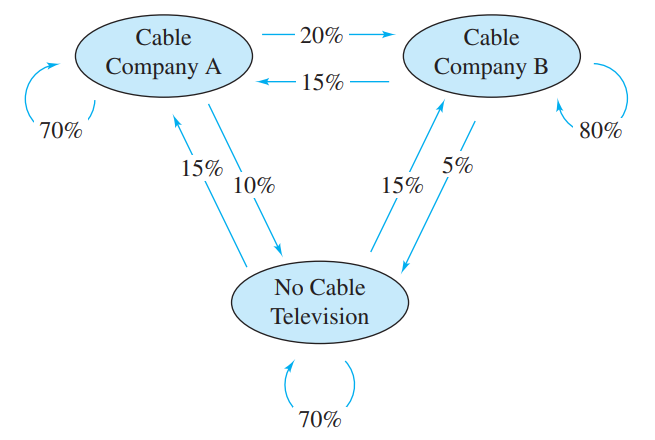
\includegraphics[width = 8cm]{cableexample.png}
    \end{center}

    The matrix representing the give transition probabilities is\\ 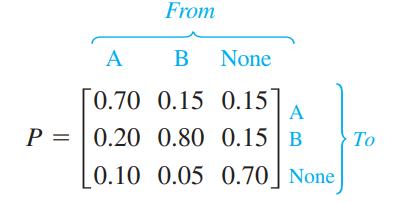
\includegraphics[width = 5cm]{ptransex.png} \\
    and the \B{state matrix} represent the current populations in 3 states is $X = \begin{bmatrix}
        15,000 \\ 20,000 \\ 65,000
    \end{bmatrix} \quad \begin{matrix}
        \text{A} \\ \text{B} \\ \text{None}
    \end{matrix}$

    The state matrix after 1 year \\
    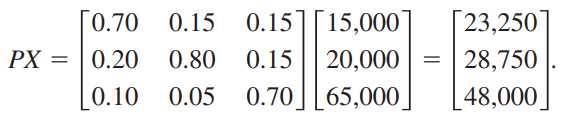
\includegraphics[width = 7cm]{ptransex1.png}

    After $n$ years: $P^nX$. But when $k$ reachs a specific value, the number of subcribers
    eventually reach a \B{steady state}. The product approaches a limit $\fillover{X}$, 
    that is $P\fillover{X} = \fillover{X}$.

    \subsection{Cryptography}

    A \B{cryptogram} is a message written according to a secret code (the Greek word \textit{kryptos} means "hidden").
    This section describes a method of using matrix multiplication to \B{encode} and \B{decode}.

    Assign a number to each letter in the alphabet. The message is converted to numbers and partitioned into \B{uncoded row matrices},
    each having $n$ entries.
    
    \subsubsection*{Forming Uncoded Row Matrices}
    Write the encoded row matrices of size $1 \x 3$ for the message MEET ME MONDAY.
    
    Partitioning the message into into groups of 3.
    \begin{center}
        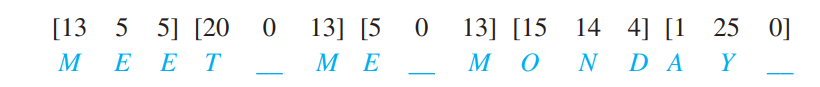
\includegraphics[width = 10cm]{uncodedrowmatrix0.png}
    \end{center}
    \begin{itemize}
        \item \textbf{Encode}: Choose an $n \x n$ invertible matrix $A$ and multiply the uncoded row matrices ($gA$).
        \item \textbf{Decode}: Multiply by $A^{-1}$. For those who do not know $A$, this is difficult.
    \end{itemize}

    \subsection{Leontief Input-Output Models}

    Suppose that an economic system has $n$ different industries $I_1, I_2, \dots, I_n$, each of which has
    \B{input} needs (raw materials, utilities, etc.) and \B{output} (finished product). In producting
    each unit of output, an industry may use the outputs of others (including itself).

    \textbf{The input-output} matrix :
    \begin{center}
            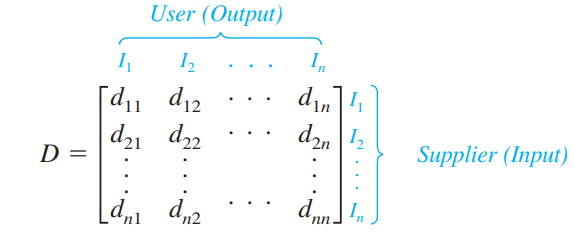
\includegraphics[width = 6cm]{inputoutput.png}
    \end{center}
    where $0 \leq d_{ij } \leq 1$ is the amount of output of the $j$th industry needs from the $i$th one to produce 1 unit
    of output per year. Sum of all entries in each column does not exceed $1$.

    If the system is \B{closed}, let the total output of the $i$th industry be denoted by $x_i$.
    \[ x_i = d_{i1}x_1 + d_{i2}x_2 + \dots + d_{in}x_n \text{(closed system)}  \]
    On the other hand, if the industries within the system sell products to nonproducing groups
    (such as goverments or charitible organizations) outside the system, then the system is \B{open}
    \[ x_i = d_{i1}x_1 + d_{i2}x_2 + \dots + d_{in}x_n + e_i \text{(closed system)}  \]
    where $e_i$ represents the external demand for the $i$th industry's product.

    The matrix form of this system is
    \begin{center}
        \begin{tcolorbox}[hbox,    %%<<---- here%
       colback = {blue9}]
       $X = DX + E$
\end{tcolorbox}
    \end{center}
    where $X$ is the \B{output matrix} and $E$ is the \B{external demand matrix}.

    \begin{equation*}
        (I - D)X = E
    \end{equation*}
    Applying Gauss-Jordan elimination on $(I - D) | E$ to solve for $x$.

    \subsection{Least Squares Regression Analysis}
    Develop Linear Models in Statistic.

    One way of measuring how well $y = f(x)$ fit the given $n$ points is to compute the differences 
    between $f(x)$ and the actual $y$. (\B{sum of squared error})

    Of all possible linear models for a given data set, the one that has the best fit is defined
    to be the one that minimizes the sum of squared error. This models is called the \B{least
    squares regression line}, and the procedure for finding it is called the \B{method of least
    squares}.

    \begin{tcolorbox}
    For a set of points, the \textbf{least squares regression line} is given by the linear function
    \[f(x) = a_0 + a_1x\]
    that minimizes the sum of squared error $ [y_i - f(x_i)]^2 $.
    \end{tcolorbox}

    To find the least squares regression line for a set of points, begin by forming the system of 
    linear equations
    \begin{equation*}
       \begin{split}
           y_1 &= f(x_1) + [y_1 - f(x_1)]\\
            & \vdots \\
           y_n &= f(x_n) + [y_n - f(x_n)]
        \end{split}
    \end{equation*}  
    where the right hand term, $[y_i - f(x_i)]$ of each equation is thought of as the error in the 
    approximation of $y_i$ by $f(x_i)$. Write it as 
    \[ e_i = y_i - f(x_i)\]
    \[y_i = (a_o + a_ix_i) + e_i \]
    Now define 
    \[ Y = \begin{bmatrix}
        y_1 \\ y_2 \\ \vdots \\ y_n
    \end{bmatrix}, \quad
    X = \begin{bmatrix}
        1 & x_1 \\
        1 & x_2 \\
        \vdots & \vdots \\
        1 & x_n
    \end{bmatrix}, \quad
    A = \begin{bmatrix}
        a_0 \\ a_1
    \end{bmatrix}, \quad
    E = \begin{bmatrix}
        e_1 \\ e_2 \\ \vdots \\ e_n
    \end{bmatrix} \]
    the $n$ linear equations may be replaced by the matrix equation
    \[Y = XA + E\]
    
    \begin{center}
    \begin{tcolorbox}[
        colback = {blue9}]
        For the regression model $Y = XA + E$, the coefficients of the least squares regression line are given by
        the matrix equation \[A = (X^TX)^{-1}X^TY\]
        and the sum of squared error is
        \[E^TE\]
    \end{tcolorbox}
    \end{center}


    







    

















\end{document}
